\documentclass[10pt]{beamer}

\usepackage[english]{babel}
\usepackage[utf8]{inputenc}
\usepackage{amsmath}
\usepackage{amssymb}
\usepackage[all]{xy}
\usepackage{graphicx}

%% Stuff
\renewcommand{\le}{\leqslant}
\renewcommand{\ge}{\geqslant}  % comme François le demande...
%% Algèbre
\newcommand{\clot}[1]{\bar{#1}}  % clôture algèbrique
\newcommand{\card}[1]{\# #1}  % cardinalité d'un ensemble
\DeclareMathOperator{\car}{char}  % caractéristique d'un corps
\DeclareMathOperator{\Frac}{Frac}  % corps des fractions
\newcommand{\Z}{\mathbb{Z}}  % les entiers
\newcommand{\K}{\mathbb{K}}  % un corps
\newcommand{\LK}{\mathbb{L}}  % encore un corps
\newcommand{\U}{\mathbb{U}}  % encore un corps
\newcommand{\F}{\mathbb{F}}  % un corps fini
\newcommand{\Q}{\mathbb{Q}}  % les rationnels
\newcommand{\R}{\mathbb{R}}  % les réels
\newcommand{\C}{\mathbb{C}}  % les complexes
\newcommand{\isom}{\cong}  % isomorphisme de corps
\newcommand{\frob}{\varphi}  % fröbenius
\DeclareMathOperator{\Gal}{Gal}  % groupe de Galois
\DeclareMathOperator{\Tr}{Tr}  % trace
\DeclareMathOperator{\PTr}{PTr}  % pseudotrace
\DeclareMathOperator{\Norm}{N} % norme
\newcommand{\euler}{\varphi}  % indicatrice d'Euler
\DeclareMathOperator{\ord}{ord}  % l'ordre d'un élément
\newcommand{\AS}[1]{\mathcal{#1}}  % la police des polynômes d'AS
\DeclareMathOperator{\rev}{rev}  % le reverse d'un polynôme
%% Courbes
\DeclareMathOperator{\Jac}{Jac}  % la jacobienne
\newcommand{\Proj}{\mathbb{P}}  % espace projectif
\newcommand{\0}{\mathcal{O}}  % point de base d'une courbe
\newcommand{\ecpoint}[3]{[#1:#2:#3]}  % un point d'une courbe
\newcommand{\isog}[1]{\mathcal{#1}}  % la police des isogénies
\newcommand{\I}{\isog{I}}  % une isogénie I
\newcommand{\Hasse}{H}  % l'invariant de Hasse
\newcommand{\divpol}{f}  % polynôme de division
%% Autre
\newcommand{\tildO}{\tilde{O}}  % la notation O~ qui oublie les log
\newcommand{\Mint}{\mathrm{\sf M}_\text{int}}  % fonction de multiplication
\newcommand{\Mpol}[1][]{\mathrm{\sf M}_\text{pol}^{#1}}  % fonction de multiplication
\newcommand{\Mult}[1][]{\mathrm{\sf M}_{#1}}  % fonction de multiplication
\newcommand{\Push}{\mathrm{\sf P}}  % fonction de push-down
\newcommand{\Lift}{\mathrm{\sf L}}  % fonction de lift-up
\newcommand{\Trace}{\mathrm{\sf T}}  % fonction de trace
\newcommand{\Frob}{\mathrm{\sf F}}  % fonction de frobenius itéré
\newcommand{\Ptr}{\mathrm{\sf PT}}  % fonction de pseudo-trace
\newcommand{\ModComp}{\mathrm{\sf C}}  % fonction de composition modulaire
\newcommand{\alg}[1]{\textsf{#1}}  % la police des algorithmes
\newcommand{\wrt}{\dashv}  % appartenance forte, a\wrt A signifie que a est représenté comme un élément de A
\DeclareMathOperator{\op}{op}  % une opération

\newenvironment{algorithm}[3]{\begin{center}\begin{minipage}{0.85\textwidth}
      \sf
      \rule{\textwidth}{0.2pt}\\
      \makebox[\textwidth][c]{\textbf{#1}}\\
      \rule[0.5\baselineskip]{\textwidth}{0.2pt}\\
      \textbf{Input~~} #2\\
      \textbf{Output} #3
      \smallskip
      \begin{enumerate}
}{\end{enumerate}
      \rule{\textwidth}{0.2pt}
\end{minipage}\end{center}}

% beamer-specific
%\setbeamertemplate{theorem begin}{
%  \begin{\inserttheoremblockenv}{
%      Théorème
%      \ifthenelse{\equal{\inserttheoremaddition}{}}
%		 {}
%		 {(\inserttheoremaddition)}    
		 %  \ifx\inserttheoremaddition\@empty\else\ (\inserttheoremaddition)\fi
%    }
%}

\mode<presentation>{%
  \usetheme[]{Madrid}
  \usefonttheme[onlymath]{serif}
  \usecolortheme{seahorse}
  \usecolortheme{rose}
}


\title[Isogenies for the Cryptology]{Computing isogenies in small characteristics}
\author[L.~De~Feo]{L.~De~Feo}
\institute[École Polytechnique]{École Polytechnique, Paris, France}
\date[U of Waterloo, May 22, 2009]{May 22, 2009\\CACR seminar\\University of Waterloo}


%% \AtBeginSection[]
%% {
%%   \begin{frame}<beamer>
%%     \frametitle{Plan}
%%     \tableofcontents[currentsection]
%%   \end{frame}
%% }


\begin{document}

\begin{frame}
  \titlepage
\end{frame}

%%
%%

\section{Introduction}

\begin{frame}
  \frametitle{Elliptic curves}

  \begin{columns} 
    \begin{column}{0.55\textwidth}
      \begin{block}{Elliptic curves}
        \begin{itemize}
        \item (Finite) field $\K$, with closure $\clot{\K}$,
        \item Weierstrass form: let $a,b\in\K$, 
          \[E \;:\; Y^2 = X^3 + aX + b\]
        \item $E(\K)$ set of $\K$-rational points,
        \item $E(\K)$ is a (finite) group. May be used for crypto.
        \end{itemize}
      \end{block}

      \begin{block}{$j$-invariant}
        \[j(E) = \frac{1728(4a)^3}{16(4a^3 + 27b^2)}\]
        Two elliptic curves are isomorphic over $\clot{\K}$ iff they
        have the same $j$-invariant.
      \end{block}
  
    \end{column}

    \begin{column}{0.4\textwidth}
      \begin{figure}
        \centering
        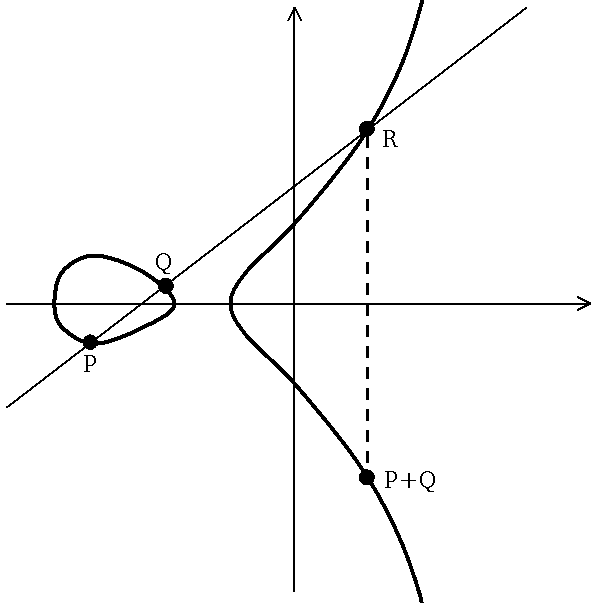
\includegraphics[width=\textwidth]{ecadd}
        \caption{point addition on an elliptic curve in Weierstrass
          form over $\R$}
      \end{figure}
    \end{column}
  \end{columns}
\end{frame}

%%

\begin{frame}
  \frametitle{Arithmetics of elliptic curves}

  \begin{block}{Multiplication}
    \begin{itemize}
    \item $[m]P = \underbrace{P + P + \cdots + P}_{m \text{ times}}$
      \hfill $[m](X,Y) = \left(\frac{\phi_m(X,Y)}{\psi_m^2(X,Y)},
      \frac{\omega_m(X,Y)}{\psi_m^3(X,Y)}\right)\quad$
    \item $\psi_m\;$ is the $m$-division polynomial, $\;\deg_X
      \psi^2\approx m^2$
    \end{itemize}
  \end{block}

  \begin{block}{Torsion}
    \begin{itemize}
    \item $E[m] \isom (\Z/m\Z)\times(\Z/m\Z)$ if $m$ prime to the
      characteristic $p$
    \item $E[p^k] \isom \begin{cases}
	\Z/p^k\Z &\text{\emph{ordinary} case}\\
	\{\0\} &\text{\emph{supersingular} case}
      \end{cases}$
    \end{itemize}
  \end{block}
\end{frame}

%%

\begin{frame}
  \frametitle{Counting points I: Schoof's algorithm}
  
  \begin{theorem}[Hasse]
    \begin{itemize}
    \item $E\;$ defined over $\;\F_q$,
    \item$\;\frob \;:\; (X,Y) \mapsto (X^q,Y^q)\;$ is the
      \emph{Frobenius morphism},
    \item its minimal polynomial is $\;\frob^2-[t]\circ\frob + [q]\;$,
    \item then $\;\card{E(\F_q)} = q + 1 - t$.
    \end{itemize}
  \end{theorem}

  \begin{block}{Computing $t$ (\cite{Scho95})}
    \begin{itemize}
    \item Modular algorithm: compute $t \bmod \ell$ for small primes
      $\ell < O(\log q)$ and compose by CRT.
    \item Let $\;P\in E[\ell]$, then
      $\quad\begin{aligned}
        &\psi_\ell(P) = 0\\
        &\frob^2(P) + [q\bmod\ell]P = [t \bmod \ell]\frob(P)
      \end{aligned}$
    \item try all $t\in[0,\ldots,\ell-1]$ until the equation is verified,
    \item to keep complexity low, work modulo the $\ell$-division
      polynomial.
    \end{itemize}
  \end{block}

\end{frame}

%%

\begin{frame}
  \frametitle{Isogenies}

  \frametitle{Isogenies}
  
  \centering $\xymatrix{ E(\clot{\K}) \ar[r]^\I & E'(\clot{\K})}$

  \begin{block}{Isogeny}
    \begin{itemize}
    \item Rational map: $\qquad \I(X,Y) =
      \left(\frac{a(X,Y)}{b(X,Y)},\frac{c(X,Y)}{d(X,Y)} \right)$,
    \item onto, finite kernel, $\qquad\deg\I = [\clot{\K}(E'):\I^\ast
      \clot{\K}(E)]$,
    \item separable, inseparable, purely inseparable like
      $\qquad \clot{\K}(E')/\I^\ast \clot{\K}(E)$,
    \item group morphism: $\qquad \I(P+Q) = \I(P) + \I(Q),\quad \I(\0_E)
      = \0_{E'}$
    \end{itemize}
  \end{block}

  \begin{block}{Examples}
    \begin{overprint}
      \onslide<1>
      Multiplication
      \begin{align*}
	[m] : E(\clot{\K}) &\rightarrow E(\clot{\K})\\
	                   P &\mapsto [m]P
      \end{align*}
      separable if and only if $\;(m,p)=1$, $\;\deg [m] = m^2$,
      $\;\ker\I = E[m]$,

      \onslide<2|handout:0>
      \emph{Small} Frobenius map
      \begin{align*}
	\frob_p : E(\clot{\K}) &\rightarrow E^{(p)}(\clot{\K})\\
	                   (X,Y) &\mapsto (X^p,Y^p)
      \end{align*}
      where $\;\;E^{(p)} \;:\; Y^2 + = X^3 + a^pX + b^p\qquad$ if $p =
      \car(\K)$,\\
      purely inseparable, $\;\deg \frob_p = p$, $\;\ker\frob_p = \{\0\}$.
 
      \onslide<3|handout:0>
      Frobenius endomorphism
      \begin{align*}
	\frob_q : E(\clot{\K}) &\rightarrow E(\clot{\K})\\
	                   (X,Y) &\mapsto (X^q,Y^q)
      \end{align*}
      if $\K = \F_q$ then $E^{(q)} = E$,\\
      purely inseparable, $\;\deg \frob_q = q$, $\;\ker\frob_q = \{\0\}$.

      \onslide<4|handout:0>
      Separable isogenies
      \[\quad\I(X,Y) = \left(\frac{g(X)}{h^2(X)},
      Y\left(\frac{g(X)}{h^2(X)}\right)'\right)\]
      separable, $\;\deg\I = \card{\ker\I} \approx \deg h$.
    \end{overprint}
  \end{block}
\end{frame}

%%

\begin{frame}
  \frametitle{Dual isogeny}

  \[\xymatrix{
    E \ar[r]^\I \ar[dr]_{[m]} & E'\ar[d]^{\hat\I}\\
    & E
  }\]

  \begin{theorem}[Dual isogeny]
    $\I$ of degree $m$, there is an unique \emph{dual isogeny}
    $\hat\I$ s.t.
    \begin{align*}
      \hat\I\circ\I &= [m]_E\\
      \I\circ\hat\I &= [m]_{E'}
    \end{align*}
  \end{theorem}

  \begin{block}{Examples}
    \begin{itemize}
    \item $[p] = V\circ\frob_p$, $\quad V$ separable,
    \item $m$ prime to $p$, $\quad [m] =  \hat\I\circ\I\quad$ separable.
    \end{itemize}
  \end{block}
\end{frame}

%%

\begin{frame}
  \frametitle{Modular polynomials}
  
  \begin{theorem}
    Let $\;H\;$ be a $\K$-rational finite subgroup of $\;E$, then
    there is an unique curve $\;E'\;$ \alert{defined over $\;\K\;$}
    and a separable isogeny $\;\I:E\rightarrow E'$ having kernel
    $\;H$.
    \[\xymatrix{
      0 \ar[r] & H \ar[r] & E \ar[r]^{\I} & E'\ar[r] & 0
    }\]
    We note $E/H$ for $E'$.
  \end{theorem}

  \begin{block}{Modular polynomial $\;\Phi_\ell(X,Y)$}
    \begin{itemize}
    \item $E[\ell] = \Z/\ell\Z\times\Z/\ell\Z\;$ contains $\;\ell+1\;$
      cyclic subgroups of order $\;\ell$,
    \item there are $\;\ell+1\;$ elliptic $j$-invariants (not necessarily
      in $\K$) $\ell$-isogenous to $E$,
    \item $\;\Phi_\ell(X,Y)$ : minimal polynomial of the \emph{modular
      function} $j(\ell\tau)$,
    \item $\Phi_\ell(j(E),j(E')) = 0\;$ iff $E$ and $E'$ are
      $\ell$-isogenous,
    \item $\deg\Phi_\ell = \ell+1$, (huge) integer coefficients.
    \end{itemize}
  \end{block}
\end{frame}

%%

\begin{frame}
  \frametitle{Counting points II : SEA (see \cite{Scho95})}
  
  \begin{block}{Schoof}
    \begin{itemize}
    \item $\frob^2 - [t]\circ\frob + [q] = 0$, compute
      $\;t\bmod\ell\;$ for primes $<O(\log q)$,
    \item computations done modulo division polynomial of degree
      $O(\ell^2)$.
    \end{itemize}
  \end{block}

  \begin{block}{Elkies}
    \begin{itemize}
    \item $E[\ell]\;$ contains subgroups $\;E_i\;$ of order $\ell$,
    \item if $\;E_1\;$ defined over $\;\K$, find isogenous curve
      $\;E/E_1$,
    \item compute $\;\I:E\rightarrow E/E_1$, then $\;\deg\I = O(\ell)$,
    \item consider $\;\frob_{E_1}$ to find $\;t\bmod\ell$,
      computations done modulo $\;\I$.
    \item Works for half of the primes.
    \end{itemize}
  \end{block}

  \begin{block}{Atkin}
    \begin{itemize}
    \item Works for the other half the of primes,
    \item uses simpler equation (in a field extension)
      $\;\frob_{E_1}=[k]_{E_1}$.
    \end{itemize}
  \end{block}
\end{frame}

%%

\begin{frame}
  \frametitle{Other applications}
  
  \begin{block}{Cryptanalysis}
    \begin{itemize}
    \item Proving hardness of discrete logarithm.
    \item Move discrete logarithms to easier curves (\cite{GHS}).
    \item Discrete logarithms in genus $3$ (\cite{Ben}).
    \end{itemize}
  \end{block}
  
  \begin{block}{Cryptography}
    \begin{itemize}
    \item Speeding up point multiplication.
    \item Hide weak curves behind chains of isogenies (\cite{Tes06}).
    \item Define hash functions.
    \end{itemize}
  \end{block}
\end{frame}

%%
%%

\section{Computing isogenies}

\begin{frame}
  \frametitle{Computing isogenies: which problem?}
  
  \begin{itemize}
  \setlength{\itemsep}{1em}
  \item Is there a $\K$-rational isogeny between $E$ and $E'$?
    \hfill\only<2->{\textcolor{blue}{$\Leftrightarrow \#E(\K) = \#E'(\K)$}}
  \item Is there a degree $\ell$ isogeny between $E$ and $E'$?
    \hfill\only<3->{\textcolor{blue}{$\Leftrightarrow \Phi_\ell(j(E), j(E')) = 0$}}
  \item What are the curves $\ell$-isogenous to $E$?
    \hfill\only<4->{\textcolor{blue}{factor $\Phi_\ell(j(E), Y)$}}
  \item Given $E$ and a subgroup $H$, find $E/H$ and $\I:E\rightarrow
    E'$ \hfill\only<5->{\textcolor{blue}{Velu formulae}}
  \item Given $E$ and a prime $\ell$, find $E'$ $\ell$-isogenous to
    $E$ and $\I:E\rightarrow E'$.
  \item \alert<6>{Given $E$, $E'$ and $\ell$, find, if it exists, an isogeny
    $\I:E\rightarrow E'$.}
  \end{itemize}

\end{frame}

%%

\begin{frame}
  \frametitle{Computing isogenies: short history}
  
  \begin{block}{Large characteristic (see \cite{BoMoSaSc08})}
    \begin{itemize}
    \item['92] Elkies \hfill $O(\ell^2)$
    \item['92] Atkin \hfill $O(\ell\Mult(\ell))$
    \item['98] Elkies \hfill $O(\ell^2)$
    \item['08] Bostan, Morain, Salvy, Schost \hfill $O(\Mult(\ell))$
    \end{itemize}
  \end{block}

  \begin{block}{Small characteristic}
    \begin{itemize}
    \item['94] Couveignes I \hfill $O(\ell^3)$
    \item['96] $p=2$, Lercier \hfill $O(\ell^3)$
    \item['96] Couveignes II (+ \cite{DF07}) \hfill $O(\ell\Mpol(\ell))$
    \end{itemize}
  \end{block}
\end{frame}

%%

\begin{frame}
  \frametitle{Computing isogenies: Couveignes II}
  
  \begin{block}{Interpolating an isogeny}
    \begin{columns}
      \begin{column}{0.3\textwidth}
        \begin{itemize}
        \item $G\;$ a \emph{large enough} subgroup,
        \item $G'\;$ its image by $\;\I$,
        \item interpolate over the points of $\;G$,
        \item deduce the isogeny by rational reconstruction.
        \end{itemize}
      \end{column}
      \begin{column}{0.7\textwidth}
        \[\xymatrix{
          E(\clot{\F}_q) \supset G \ar[rr]^\I &&
          G' \subset E'(\clot{\F}_q)
        }\]
        \[\xymatrix{
          \ar@{=>}[d]  \\
          A(X_P) = A(X_{P'}) \quad
          \text{for every $P\in G$, $P'=\I(P)$}
        }\]
        \[\xymatrix{
          \ar@{=>}[d] \\
          \frac{g(X)}{h^2(X)}
        }\]
      \end{column}
    \end{columns}
  \end{block}
  
  \begin{center}
    $G\;$ is chosen to be $\;E[p^k]$
  \end{center}
\end{frame}

%%

\begin{frame}
  \frametitle{Intermezzo : $p$-torsion of ordinary elliptic curves}
  
  \begin{block}{$p^k$-torsion}
    \begin{itemize}
    \item $E[p^k]\;$ cyclic group isomorphic to $\;\Z/p^k\Z$,
    \item $\I(E[p^k]) = E'[p^k]\;$ if $\;(\ell,p)=1$,
    \item points not necessarily defined over $\K$.
    \end{itemize}
  \end{block}

  \begin{block}{$p^k$-torsion tower}
    $(\K = \U_0, \ldots, \U_k)$ is the tower of field extensions of minimal
    degree s.t. for any $i$
    \[E[p^i] \subset E(\U_i)\text{.}\]
  \end{block}

  \begin{block}{Remark (Structure of $(\U_0, \ldots, \U_k)$)}
    There is a $i_0$ s.t. $\U_{i_0} = \U_0$ and for $i \ge i_0$
    \begin{center}
      $[\U_{i+1}:\U_i] = p$,
    \end{center}
  \end{block}
\end{frame}

%%
%%

\section{Methods}

\begin{frame}
  \frametitle{Methods I : Artin-Schreier towers}

  \begin{definition}[Artin-Schreier polynomial]
    $\K$ a field of characteristic $p$, $\alpha\in\K$
    \[X^p - X - \alpha\]
    is an Artin-Schreier polynomial.
  \end{definition}
  
  \begin{theorem}
    $\K$ finite. $X^p - X - \alpha$ irreducible $\Leftrightarrow \;
    \Tr_{\K/\F_p}(\alpha) \ne 0$.\\ If $\eta\in\K$ is a root, then $\eta
    + 1, \ldots, \eta + (p-1)$ are roots.
  \end{theorem}
  
  \begin{definition}[Artin-Schreier extension]
    $\AS{P}$ an irreducible Artin-Schreier polynomial. 
    \[\LK = \K[X]/\AS{P}(X) \text{.}\]
    $\LK/\K$ is called an Artin-Schreier extension.
  \end{definition}
\end{frame}

%%

\begin{frame}
  \frametitle{Methods I : Artin-Schreier towers}

  \begin{columns}
    \begin{column}{0.3\textwidth}
      \Large\[\xymatrix{
        *+[r]{\U_k = \frac{\U_{k-1}[X_k]}{P_{k-1}(X_k)}}\ar@{-}[d]^p\\
        *+[r]{\U_{k-1}} \ar@{--}[dd]\\
        \\
        *+[r]{\U_1 = \frac{\U_0[X_1]}{P_0(X_1)}} \ar@{-}[d]^p\\
        *+[r]{\U_0 = \F_{p^d} = \frac{\F_p[X_0]}{Q(X_0)}}
      }\]
    \end{column}
    \begin{column}{0.65\textwidth}
      \begin{block}{Towers over finite fields}
        \smallskip
        \begin{center}
          \Large$P_i = X^p - X - \alpha_i$
        \end{center}
        \vfill
        \begin{center}
          We say that $(\U_0,\ldots,\U_k)$ is defined by
          $(\alpha_0,\ldots,\alpha_{k-1})$ over $\U_0$.
        \end{center}
        \begin{center}
          \alert{ANY} separable extension of degree $p$ can be
          expressed this way
        \end{center}
      \end{block}

      \begin{block}{Voloch formulae}
        Given $\;E$, compute $\;(\alpha_0,\ldots,\alpha_{k-1})\;$ that
        define the $p^k$-torsion tower of $\;E$.
      \end{block}
    \end{column}
  \end{columns}
\end{frame}

%%

\begin{frame}
  \frametitle{Methods II : Fast arithmetics in Artin-Schreier towers}

  \begin{columns}
    \begin{column}{0.1\textwidth}
      \Large\[\xymatrix{
        \U_k\ar@{-}[d]\\
        \U_{k-1} \ar@{--}[dd]\\
        \\
        \U_1 \ar@{-}[d]\\
        \U_0
      }\]
    \end{column}
    \begin{column}{0.85\textwidth}
      \begin{block}{Primitive towers (\cite{DFS09})}
        \begin{itemize}
        \item Find special towers s.t. $\;\U_i = \F_p[X_i]$, where
          $\;X_i^p-X_i-\alpha_{i-1}=0$,
        \item use polynomial basis to perform fast arithmetics (FFT
          multiplication, Newton inversion, etc.),
        \item generalise to any tower using isomorphism algorithms.
        \end{itemize}
      \end{block}
      
      \begin{block}{Level embedding (\cite{DFS09})}
        \begin{itemize}
        \item Express the morphisms between the levels to switch back
          to the multivariate representation.
        \item Going down is easy: bivariate reduction modulo
          $X_i^p-X_i-\alpha_{i-1}$.
        \item Going up much harder:
          \begin{itemize}
          \item trace formulae,
          \item truncated power series arithmetics,
          \item transposition principle.
          \end{itemize}
        \end{itemize}
      \end{block}
    \end{column}
  \end{columns}
\end{frame}

%%

\begin{frame}
  \frametitle{Intermezzo : duality and transposition principle}

  \begin{center}
    ``From every \emph{linear algorithm} computing a
    linear application we can deduce another \emph{linear algorithm}
    computing the transpose application using \emph{about} the same
    space and time resources.''
  \end{center}

  \begin{block}{Category theory justification}
    \Large
    \[\xymatrix{
      & \ar[r]\ar@{}[dr]|{C_2} & \ar[dr] &
      & \ar[r]\ar@{}[dr]|{C_1} & \ar[dr] \\
      a \ar[ur]\ar@{-->}[rrr]_{f_2} &&& b
      \ar[ur]\ar@{-->}[rrr]_{f_1} &&& c
    }\]
  \end{block}
\end{frame}

%%

\begin{frame}
  \frametitle{Methods III : beyond fast interpolation (\cite{DF07})}
  
  \begin{columns}
    \begin{column}{0.01\textwidth}
    \end{column}
    \begin{column}{0.149\textwidth}
      \begin{center}
	Subproduct tree
      \end{center}
    \end{column}

    \begin{column}{0.85\textwidth}
      \tiny
      \hfill
      \xymatrix@R=0pt@C=14pt{
        \\
	& & & **[r](X - [p^k - 1]P)\ar@{-}"3,3"_-{\times} \\
	& & U_{1,p^{k-1}}\ar@{.}"4,2" & {\vdots} \\
	& U_{k-1,p}\ar@{-}"7,1"_{\times} & & **[r](X-[p^k-p+2]P)\ar@{-}"3,3"_-{\times} \\
	& & {\vdots} & **[r](X - [p^k-p+1]P)\ar@{-}"3,3"^-{\times} \\
	& {\vdots} & & {\vdots} \\
    T_k & & & **[r](X - [2p - 1]P)\ar@{-}"8,3"_-{\times} \\
	& U_{k-1,2}\ar@{-}"7,1"_{\times} & U_{1,2}\ar@{.}"10,2" & {\vdots} \\
	& & & **[r](X-[p+2]P)\ar@{-}"8,3"_-{\times}  \\
	& U_{k-1,1}\ar@{-}"7,1"^{\times} & & **[r](X - [p+1]P)\ar@{-}"8,3"^-{\times} \\
	& & & **[r](X - [p-1]P)\ar@{-}"12,3"_-{\times}  \\
	& & U_{1,1}\ar@{.}"10,2" & {\vdots} \\
	& & & **[r](X - [2]P)\ar@{-}"12,3"_-{\times}  \\
	& & & **[r](X - P)\ar@{-}"12,3"^-{\times}
      }
    \end{column}
  \end{columns}
\end{frame}

%%

\begin{frame}<1-3>
  \frametitle{Methods III : beyond fast interpolation (\cite{DF07})}
  
  \footnotesize

  \begin{columns}
    \begin{column}{0.3\textwidth}
      \normalsize
      $p^k$-torsion tree
    \end{column}
    \begin{column}{0.7\textwidth}
      \tiny

      \[\xymatrix@R=0pt@C=25pt{
	{\U_0 \ar@{-}[r]} & {\U_1 \ar@{.}[r]} &
	{\U_{k-1} \ar@{-}[r]} & {\U_k}
	\\
	& & & **[r](X - P_n)^{\frob^{p-1}_{k-1}}\ar@{-}"3,3"_-{\times} \\
	& & \alt<1>{U_{1,n}^{\phantom{\frob_{k-2}^{p-1}}}}{U_{1,m}^{\frob_{k-2}^{p-1}}}\ar@{.}"4,2" & {\vdots} \\
	& \alt<1-2>{U_{k-1,p-1}^{\phantom{\frob_0^{p-1}}}}{U_{k-1,1\phantom{-p}}^{\frob_0^{p-1}}}\ar@{-}"7,1"_{\times} & & **[r](X-P_n)^{\frob_{k-1}}\ar@{-}"3,3"_-{\times} \\
	& & {\vdots} & **[r](X - P_n)\ar@{-}"3,3"^-{\times} \\
	& & & \\
    T_k & & & **[r](X - P_2)^{\frob^{p-1}_{k-1}}\ar@{-}"8,3"_-{\times} \\
	& \alt<1-2>{U_{k-1,2}^{\phantom{\frob_0}}}{U_{k-1,1}^{\frob_0}}\ar@{-}"7,1"_{\times} & \alt<1>{U_{1,2}^{\phantom{\frob_{k-2}}}}{U_{1,1}^{\frob_{k-2}}}\ar@{.}"10,2" & {\vdots} \\
	& & & **[r](X-P_2)^{\frob_{k-1}}\ar@{-}"8,3"_-{\times}  \\
	& U_{k-1,1}\ar@{-}"7,1"^{\times} & & **[r](X - P_2)\ar@{-}"8,3"^-{\times} \\
	& & & **[r](X - P_1)^{\frob^{p-1}_{k-1}}\ar@{-}"12,3"_-{\times}  \\
	& & U_{1,1}\ar@{.}"10,2" & {\vdots} \\
	& & & **[r](X - P_1)^{\frob_{k-1}}\ar@{-}"12,3"_-{\times} \\
	& & & **[r](X - P_1)\ar@{-}"12,3"^-{\times}
      }\]
    \end{column}
  \end{columns}
\end{frame}

%%
%%

\begin{frame}
  \frametitle{Bibliography}

  \begin{thebibliography}{1}
    \beamertemplatebookbibitems
    
  \bibitem[BSS1]{BSS1} I.~Blake, G.~Seroussi \& N.~Smart
    \newblock \emph{Elliptic Curves in Cryptography}
    \newblock LMS 265, Cambridge University Press, 1999
    
  \bibitem[BSS2]{BSS2} (edited by) I.~Blake, G.~Seroussi \& N.~Smart
    \newblock \emph{Advances in Elliptic Curve Cryptography}
    \newblock LMS 317, Cambridge University Press, 2005
        
  \bibitem[Mil]{MIL} J.S.~Milne.
    \newblock \emph{Elliptic curves}.
    \newblock BookSurge Publishers, ISBN 1-4196-5257-5, 2006.

  \bibitem[Sil]{SIL1} J.H.~Silverman
    \newblock \emph{The Arithmetic of Elliptic Curves}
    \newblock GTM 106, Springer-Verlag, 1986
        
  \end{thebibliography}
\end{frame}

\begin{frame}
  \frametitle{Bibliography}

  \begin{thebibliography}{1}
    \beamertemplatearticlebibitems
    
  \bibitem[Bostan, Morain, Salvy, Schost 08]{BoMoSaSc08} A.~Bostan,
    F.~Morain, B.~Salvy, É.~Schost.  \newblock Fast algorithms for
    computing isogenies between elliptic curves.
    \newblock \emph{Math. Comp.} 77, 263, 1755-1778, 2008.
    
  \bibitem[Couveignes '96]{Cou96}J.-M.~Couveignes.
    \newblock Computing $\ell$-isogenies with the $p$-torsion.
    \newblock \emph{Lecture Notes in Computer Science} vol. 1122, pages 59--65,
    Springer-Verlag, 1996.
    
  \bibitem[Couveignes '00]{Couveignes00} J.-M. Couveignes.
    \newblock Isomorphisms between {A}rtin-{S}chreier tower.
    \newblock \emph{Math. Comp.} 69(232): 1625--1631, 2000.

  \bibitem[D.F. '07]{DF07} L.~De~Feo.  \newblock Calcul d'isogénies.
    \newblock Master
    thesis. \href{http://www.lix.polytechnique.fr/~defeo/papers/master.pdf}{http://www.lix.polytechnique.fr/$\sim$defeo}

  \bibitem[D.F., Schost '09]{DFS09} L.~De~Feo \& É.~Schost.  \newblock
    Fast arithmetics in Artin-Schreier towers over finite fields.
    \newblock \emph{Preprint}, 2009.

  \end{thebibliography}
\end{frame}


\begin{frame}
  \frametitle{Bibliography}

  \begin{thebibliography}{1}

  \bibitem[Gaudry, Hess, Smart '02]{GHS}
    P.~Gaudry, F.~Hess, N.~P.~Smart.
    \newblock Constructive and destructive facets of Weil
    descent on elliptic curves.
    \newblock \emph{J. Cryptology} 15:19-46, 2002.

  \bibitem[Schoof '95]{Scho95} R.~Schoof. \newblock Counting points on
    elliptic curves over finite fields. \newblock \emph{J. de Théorie
      des Nombres de Bordeaux}, 7:219-254, 1995.

  \bibitem[Smith '08]{Ben} B.~Smith.  \newblock Isogenies and the
    Discrete Logarithm Problem in Jacobians of genus $3$ hyperelliptic
    curves.
    \newblock In \emph{EUROCRYPT '08}, LNCS, 2008.

  \bibitem[Teske '06]{Tes06} E.~Teske. \newblock Elliptic curve
    trapdoor system. \newblock \emph{J. Cryptology} 19:115-133, 2006.

  \end{thebibliography}
\end{frame}




\end{document}


% Local Variables:
% mode:flyspell
% ispell-local-dictionary:"british"
% End:
%

% LocalWords:  Isogeny abelian isogenies hyperelliptic supersingular Frobenius
% LocalWords:  isogenous
